\section{Stylized facts and correlation structure}
\label{sec:stylized_correlation}

\subsection{Stylized facts of selected B3 assets}

Figure~\ref{fig:stylized_facts} summarises the return properties of PETR4, VALE3 and BBDC4. We use these assets as representative examples and as the initial forecasting targets because they are liquid, economically important and sectorally distinct; they are not intended to be a proxy for the entire Brazilian equity market. The figure combines four checks that are standard in the econophysics literature \cite{cont_2001_empirical}: normalized prices, daily returns, the complementary cumulative distribution of absolute returns and the autocorrelation of absolute returns.

\begin{center}

\includegraphics[width=0.95\linewidth]{images/figure_1d_stylized_facts_demo_assets_clean_2006_2025.pdf}
\captionof{figure}{Stylized facts for PETR4, VALE3 and BBDC4 over 2006--2025. The panels show normalized prices, daily log returns, the complementary cumulative distribution of absolute returns and autocorrelations of absolute returns. The return panel uses three vertically aligned subpanels with a common scale and a zero reference line for each asset.}
\label{fig:stylized_facts}
\end{center}

The normalized-price panel illustrates heterogeneous long-run trajectories across the three assets. This heterogeneity is expected because the selected firms belong to distinct economic segments and are exposed to different sectoral and macro-financial drivers. The return panel displays periods in which large movements cluster over time, a pattern indicating volatility clustering. The CCDF panel suggests that large absolute returns occur more frequently than would be expected under a Gaussian benchmark, pointing to heavy-tailed returns. The autocorrelation panel shows positive dependence in $|r_t|$ over several lags, indicating persistent volatility \cite{cont_2001_empirical}.

\subsection{Descriptive statistics}

Table~\ref{tab:descriptive_stats} quantifies the same diagnostics. All three series have means close to zero, substantial kurtosis and non-negligible counts of large absolute returns. PETR4 has the largest negative daily observation in the 2006--2025 window, while VALE3 and BBDC4 also show stress-period extremes. The autocorrelations of absolute returns remain positive across several lags, especially for VALE3.

The descriptive statistics match the visual reading of Figure~\ref{fig:stylized_facts}. The return distributions display substantial departures from a Gaussian benchmark, including excess kurtosis and persistent absolute-return autocorrelations. These properties match the well-documented stylized facts of financial returns \cite{cont_2001_empirical} and support treating the Brazilian market as a complex system in which dependency structure, not marginal normality, is the relevant modelling object.

\begin{center}
\captionof{table}{Descriptive statistics for the three demonstration assets, 2006--2025.}
\label{tab:descriptive_stats}
\scriptsize
\setlength{\tabcolsep}{2.8pt}
\resizebox{\linewidth}{!}{%
\begin{tabular}{lrrrrrrrrrrrrrrr}
\toprule
Symbol & $n$ & Mean & Std. & Skew. & Ex. kurt. & Min. & Max. &
VaR$_{1\%}$ & VaR$_{5\%}$ &
$|r|>10\%$ & $|r|>20\%$ &
ACF$_1$ & ACF$_5$ & ACF$_{20}$ & ACF$_{60}$ \\
\midrule
BBDC4 & 4953 & 0.00028 & 0.02180 &  0.02 &  7.96 & -0.1910 & 0.1999 & -0.0559 & -0.0312 & 16 & 0 & 0.207 & 0.174 & 0.122 & 0.044 \\
PETR4 & 4953 & 0.00041 & 0.02755 & -0.76 & 11.55 & -0.3524 & 0.2007 & -0.0767 & -0.0408 & 41 & 4 & 0.254 & 0.209 & 0.140 & 0.062 \\
VALE3 & 4953 & 0.00045 & 0.02576 & -0.22 &  7.51 & -0.2814 & 0.1936 & -0.0676 & -0.0381 & 26 & 2 & 0.231 & 0.207 & 0.169 & 0.119 \\
\bottomrule
\end{tabular}}
\end{center}

\noindent\footnotesize\emph{Notes:} Mean and Std. are the sample mean and standard deviation of daily log returns. Skew. is sample skewness and Ex. kurt. is excess kurtosis relative to the Gaussian benchmark. VaR$_{1\%}$ and VaR$_{5\%}$ are the empirical 1\% and 5\% lower-tail return quantiles. $|r|>10\%$ and $|r|>20\%$ count daily observations whose absolute log return exceeds the stated threshold. ACF$_\ell$ is the autocorrelation of absolute returns at lag $\ell$ trading days.

\normalsize

\subsection{Static correlation distribution}

We now turn from individual return behaviour to cross-sectional dependence. The core historical universe contains 58 assets, producing $N(N-1)/2=1653$ unique asset pairs. The static pairwise summaries below use the available overlap for each pair and therefore describe the broader unbalanced historical coverage; Figure~\ref{fig:correlation_structure} summarizes their distribution and then splits pairs into within-sector and between-sector groups. The subsequent RMT decomposition instead uses the single complete 58-asset panel from 23 August 2006 to 15 August 2024.

\begin{center}
\begin{minipage}{0.49\linewidth}
  \centering
  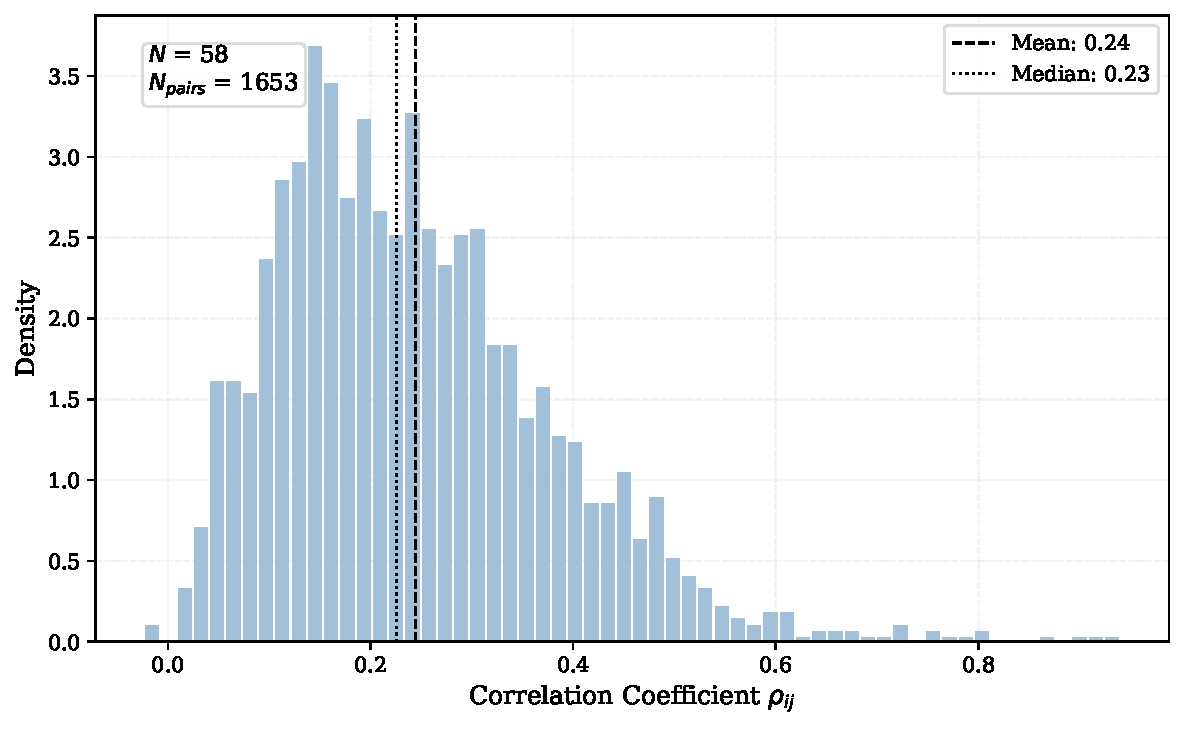
\includegraphics[width=\linewidth]{images/figure_2_correlation_histogram.pdf}
  \vspace{0.2cm}

  \small (a) Full pairwise distribution.
\end{minipage}
\hfill
\begin{minipage}{0.49\linewidth}
  \centering
  
\includegraphics[width=\linewidth]{images/figure_3_sector_correlation_distribution.pdf}
  \vspace{0.2cm}

  \small (b) Within-sector and between-sector pairs.
\end{minipage}

\captionof{figure}{Correlation structure in the core historical universe. Panel (a) shows the full Pearson correlation distribution. Panel (b) compares within-sector and between-sector correlations using the initial macro-sector classification.}
\label{fig:correlation_structure}
\end{center}

The full distribution is centred in a moderate positive range, with mean correlation close to 0.24 and median correlation close to 0.23. This level of average dependence suggests the presence of a common component, but the distribution remains dispersed. The dispersion is important because it leaves room for sectoral and subsectoral organization instead of a single homogeneous market block.

\subsection{Sectoral correlation comparison}

The sector split gives a descriptive check of this interpretation. Within-sector correlations are visibly shifted to the right relative to between-sector correlations. Table~\ref{tab:sector_corr_summary} reports the corresponding pair counts and summary statistics. These results indicate that the initial macro-sector map is reflected in the dependency matrix.

\begin{center}
\captionof{table}{Within-sector and between-sector correlation summary.}
\label{tab:sector_corr_summary}
\begin{tabular}{lrrrrrr}
\toprule
Group & Pairs & Mean & Median & Std. dev. & Min & Max \\
\midrule
Within-sector & 275 & 0.3433 & 0.3082 & 0.1819 & 0.0534 & 0.9402 \\
Between-sector & 1378 & 0.2249 & 0.2076 & 0.1166 & -0.0236 & 0.5552 \\
\bottomrule
\end{tabular}
\end{center}

The difference is economically meaningful. Within-sector pairs have mean correlation 0.3433, while between-sector pairs have mean correlation 0.2249, giving $\Delta_{\mathrm{sector}}=0.1184$. An asset-level label-permutation test with 10,000 sector-label reallocations preserves both the observed dependency matrix and the sector-size vector, without treating overlapping pairs as independent observations. None of the permuted statistics reaches the observed difference (null 95th percentile $=0.0245$; one-sided Monte Carlo $p<0.0001$). Conditional on exchangeability of sector labels under the null and on the initial macro-sector map, this provides evidence that the sectoral grouping is reflected in the dependency matrix.

\subsection{Dynamic market synchronization}

Full-sample correlations are limited because market dependence changes over time. Figure~\ref{fig:rolling_corr} shows the rolling average market correlation using 252- and 504-trading-day windows. This statistic compresses the correlation matrix into a time series that measures how synchronized the market is at each point in time. The historical panel has changing coverage in its earliest years: each window uses the assets with data available in that window, ranging from 40 assets initially to the full 58-asset universe in later periods. The series should therefore be interpreted as a descriptive measure of the average available pairwise dependence.

\begin{center}
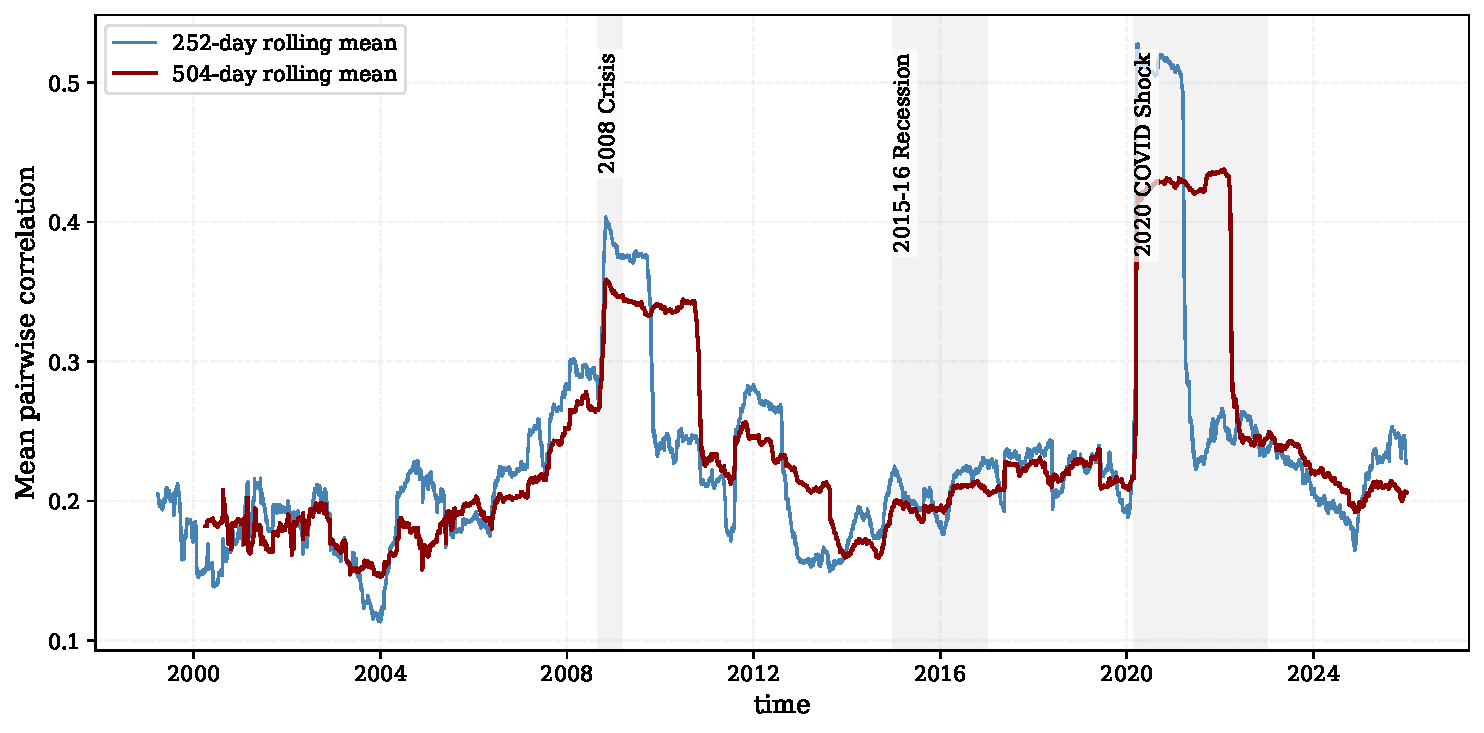
\includegraphics[width=\linewidth]{images/figure_4_rolling_average_correlation.pdf}
\captionof{figure}{Rolling average market correlation for the core historical universe, estimated with 252- and 504-trading-day windows. Each window uses the assets available during that period.}
\label{fig:rolling_corr}
\end{center}

The rolling average correlation tends to rise around major stress periods, including the 2008 global financial crisis, the Brazilian recession period around 2015--2016 and the 2020 COVID shock. These episodes indicate periods of stronger market-wide synchronization, which helps explain the dominant leading eigenvalue in the full-sample correlation matrix.

Figure~\ref{fig:dynamic_pairwise} adds a more granular view by showing selected pairwise dynamic correlations under different estimators. The pairs were selected for their economic interpretability: PETR4--VALE3 compares two large commodity-exposed firms in distinct subsectors; BBDC4--BBAS3 represents financials; GGBR4--USIM5 represents steel and metallurgy; and ELET3--CMIG4 represents utilities. The figure is illustrative rather than a representative sample of all possible pairs.

The analytical role of these estimates is to show that a single full-sample correlation can conceal episodes in which a dependency strengthens, weakens or temporarily breaks down. The 20-day Pearson estimate reacts quickly to local changes but is noisy; the 60-day estimate is smoother but slower; and EWMA with a 20-day half-life provides an intermediate adaptive estimate. Together, the three views distinguish persistent co-movement from short-lived correlation bursts. This makes the figure a useful sensitivity check for the static correlation matrix used in the subsequent RMT and network analyses: it does not replace the full matrix, but demonstrates why its resulting structures should be interpreted as long-run summaries of a time-varying dependency system.

\begin{center}

\includegraphics[width=\linewidth]{images/figure_5_dynamic_pairwise_correlations.pdf}
\captionof{figure}{Dynamic pairwise correlations for selected economically interpretable asset pairs. Pearson estimates use 20- and 60-trading-day windows; EWMA uses a 20-day half-life. The estimates show how individual dependencies can vary across time scales.}
\label{fig:dynamic_pairwise}
\end{center}
